% Copyright 2004 by Till Tantau <tantau@users.sourceforge.net>.
%
% In principle, this file can be redistributed and/or modified under
% the terms of the GNU Public License, version 2.
%
% However, this file is supposed to be a template to be modified
% for your own needs. For this reason, if you use this file as a
% template and not specifically distribute it as part of a another
% package/program, I grant the extra permission to freely copy and
% modify this file as you see fit and even to delete this copyright
% notice. 

\documentclass{beamer}

% There are many different themes available for Beamer. A comprehensive
% list with examples is given here:
% http://deic.uab.es/~iblanes/beamer_gallery/index_by_theme.html
% You can uncomment the themes below if you would like to use a different
% one:
%\usetheme{AnnArbor}
%\usetheme{Antibes}
%\usetheme{Bergen}
%\usetheme{Berkeley}
%\usetheme{Berlin}
%\usetheme{Boadilla}
%\usetheme{boxes}
%\usetheme{CambridgeUS}
%\usetheme{Copenhagen}
%\usetheme{Darmstadt}
\usetheme{default}
%\usetheme{Frankfurt}
%\usetheme{Goettingen}
%\usetheme{Hannover}
%\usetheme{Ilmenau}
%\usetheme{JuanLesPins}
%\usetheme{Luebeck}
%\usetheme{Madrid}
%\usetheme{Malmoe}
%\usetheme{Marburg}
%\usetheme{Montpellier}
%\usetheme{PaloAlto}
%\usetheme{Pittsburgh}
%\usetheme{Rochester}
%\usetheme{Singapore}
%\usetheme{Szeged}
%\usetheme{Warsaw}

\usepackage{graphicx}

\title{Presentation Title}

% A subtitle is optional and this may be deleted
\subtitle{Optional Subtitle}

\author{K.~Cong}
% - Give the names in the same order as the appear in the paper.
% - Use the \inst{?} command only if the authors have different
%   affiliation.

\institute[Delft University of Technology] % (optional, but mostly needed)
{
  Faculty of Electrical Engineering, Mathematics and Computer Science\\
  Delft University of Technology}
% - Use the \inst command only if there are several affiliations.
% - Keep it simple, no one is interested in your street address.

% \date{Conference Name, 2013}
\date{2017}
% - Either use conference name or its abbreviation.
% - Not really informative to the audience, more for people (including
%   yourself) who are reading the slides online

% \subject{Theoretical Computer Science}
% This is only inserted into the PDF information catalog. Can be left
% out. 

% If you have a file called "university-logo-filename.xxx", where xxx
% is a graphic format that can be processed by latex or pdflatex,
% resp., then you can add a logo as follows:

% \pgfdeclareimage[height=0.5cm]{university-logo}{university-logo-filename}
% \logo{\pgfuseimage{university-logo}}

% Delete this, if you do not want the table of contents to pop up at
% the beginning of each subsection:
\AtBeginSubsection[]
{
  \begin{frame}<beamer>{Outline}
    \tableofcontents[currentsection,currentsubsection]
  \end{frame}
}

% Let's get started
\begin{document}

\begin{frame}
  \titlepage
\end{frame}

\begin{frame}{Outline}
  \tableofcontents
  % You might wish to add the option [pausesections]
\end{frame}

% Section and subsections will appear in the presentation overview
% and table of contents.
\section{Background}

\subsection{TrustChain}

\begin{frame}{TrustChain}{}

  \begin{figure}[h]
  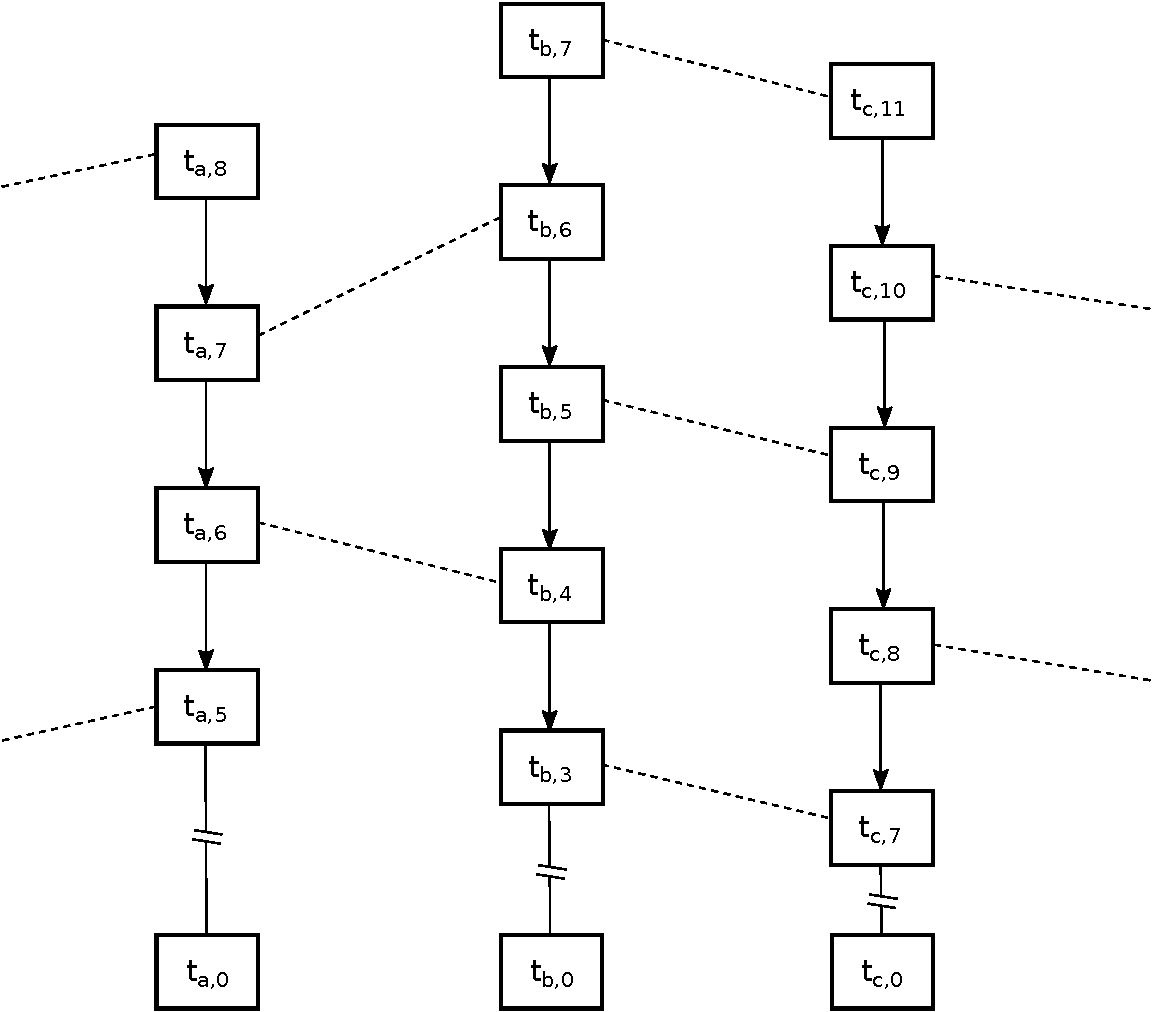
\includegraphics[width=0.7\textwidth]{figures/trustchain-good}
  \centering
  \caption{\emph{TX block} is a six-tuple: $t_{i,j} = (\texttt{h}(b_{i,j-1}),
    h_s, h_r, s_s, s_r, m)$, one transaction results in two TX blocks---\emph{a
      pair}.}
  \end{figure}

\end{frame}

\begin{frame}{TrustChain}{}

  \begin{figure}[h]
  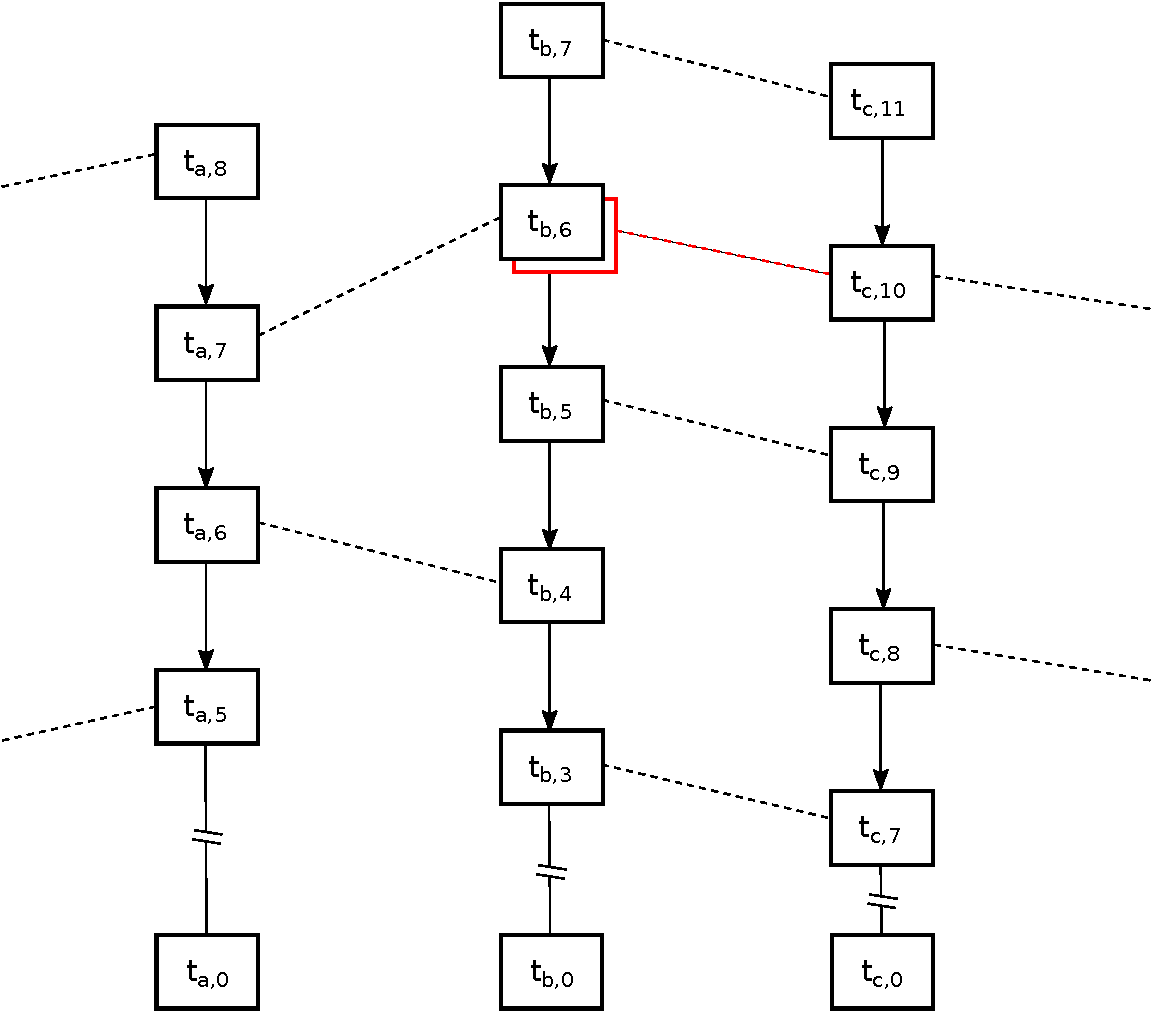
\includegraphics[width=0.7\textwidth]{figures/trustchain-bad}
  \centering
  \caption{Fork is two correctly signed TX blocks that has the same $h_s$ but
    involve different receivers. Only one TX block may be in consensus.}
  \end{figure}

\end{frame}

\begin{frame}{TrustChain}
  \begin{itemize}
    \item Everyone has their own chain
    \item Transactions are on arbitrary data $m$
    \item Transactions make the chains intertwined
    \item No consensus (my thesis)
  \end{itemize}
\end{frame}

\section{My Thesis}
\subsection{TrustChain with Checkpoints}
\begin{frame}{TrustChain with Checkpoints}

  \begin{figure}[h]
  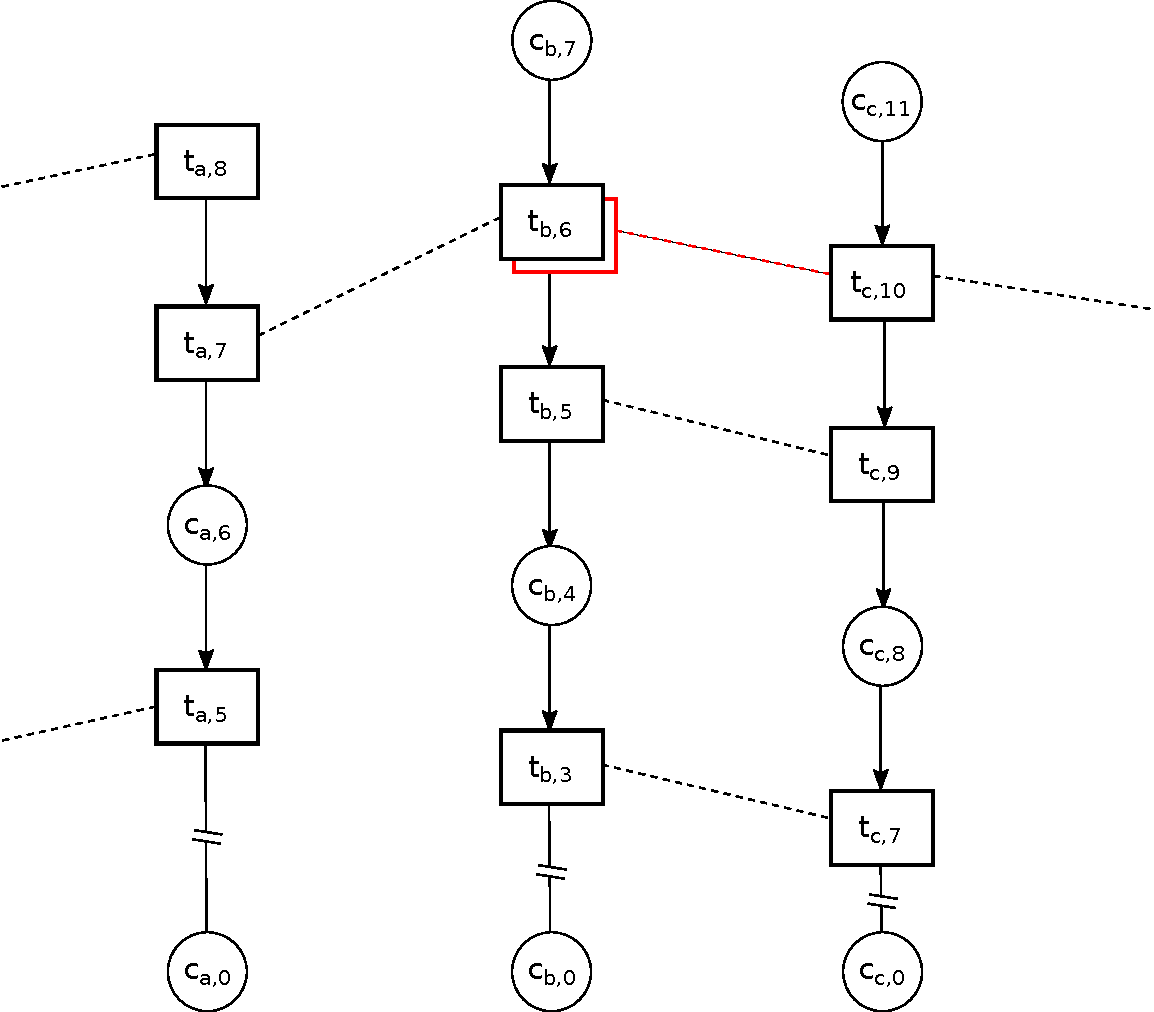
\includegraphics[width=0.7\textwidth]{figures/trustchain-bad-cp}
  \centering
  \caption{CP block is a five-tuple: $c_{i,j} = (\texttt{h}(b_{i,j-1}),
    \texttt{h}(\mathcal{C}_r), r, p, s)$, $\mathcal{C}_r$ is the consensus
    result at round $r$, $p =$ promoter indicator, $s =$ signature.}
  \end{figure}

\end{frame}

\subsection{Consensus Protocol Overview}
\begin{frame}{Consensus Protocol Overview}
  \begin{enumerate}
    \item $N$ lucky nodes are selected at random to act as promoters.
    \item Every node sends CP blocks to promoters.
    \item Promoters run a BFT (Byzantine Fault Tolerant) consensus algorithm to
      agree on a set of CP blocks---$\mathcal{C}_r$.
    \item Disseminate $\mathcal{C}_r$.
    \item Any node can verify that their transaction is in consensus.
    \item Repeat for next round.
  \end{enumerate}
\end{frame}

\subsection{Promoter Registration}
\begin{frame}{Promoter Registration}

\end{frame}

\begin{frame}{Blocks}
\begin{block}{Block Title}
You can also highlight sections of your presentation in a block, with it's own title
\end{block}
\begin{theorem}
There are separate environments for theorems, examples, definitions and proofs.
\end{theorem}
\begin{example}
Here is an example of an example block.
\end{example}
\end{frame}

% Placing a * after \section means it will not show in the
% outline or table of contents.
\section*{Summary}

\begin{frame}{Summary}
  \begin{itemize}
  \item
    The \alert{first main message} of your talk in one or two lines.
  \item
    The \alert{second main message} of your talk in one or two lines.
  \item
    Perhaps a \alert{third message}, but not more than that.
  \end{itemize}
  
  \begin{itemize}
  \item
    Outlook
    \begin{itemize}
    \item
      Something you haven't solved.
    \item
      Something else you haven't solved.
    \end{itemize}
  \end{itemize}
\end{frame}



% All of the following is optional and typically not needed. 
\appendix
\section<presentation>*{\appendixname}
\subsection<presentation>*{For Further Reading}

\begin{frame}[allowframebreaks]
  \frametitle<presentation>{For Further Reading}
    
  \begin{thebibliography}{10}
    
  \beamertemplatebookbibitems
  % Start with overview books.

  \bibitem{Author1990}
    A.~Author.
    \newblock {\em Handbook of Everything}.
    \newblock Some Press, 1990.
 
    
  \beamertemplatearticlebibitems
  % Followed by interesting articles. Keep the list short. 

  \bibitem{Someone2000}
    S.~Someone.
    \newblock On this and that.
    \newblock {\em Journal of This and That}, 2(1):50--100,
    2000.
  \end{thebibliography}
\end{frame}

\end{document}


